\documentclass[tikz,border=12pt]{standalone}
\usepackage[T1]{fontenc}
\usepackage{tgheros}
\usepackage{sfmath}
\usepackage{amsmath,amssymb}
\usepackage{fontawesome5}
\usepackage{tikz}
\usetikzlibrary{arrows.meta,positioning,shapes.geometric,fit,backgrounds,calc,decorations.pathreplacing}
\usepackage{xcolor}

\renewcommand{\familydefault}{\sfdefault}

% Academic Semantic Palette
\definecolor{ethdarkblue}{HTML}{1B2A4A}
\definecolor{ethslate}{HTML}{475569}
\definecolor{cardbg}{HTML}{F8FAFC}
\definecolor{cardborder}{HTML}{CBD5E1}
\definecolor{measuredTeal}{HTML}{168F84}
\definecolor{tealBg}{HTML}{E4F6F3}
\definecolor{proposalAmber}{HTML}{C98218}
\definecolor{amberBg}{HTML}{FFF3DC}
\definecolor{consequenceCoral}{HTML}{BD4F2F}
\definecolor{coralBg}{HTML}{FAE9E2}
\definecolor{authorityViolet}{HTML}{6550A8}
\definecolor{violetBg}{HTML}{F0ECFA}
\definecolor{crimsonDark}{HTML}{A51C30}

\begin{document}
\begin{tikzpicture}[
  font=\sffamily,
  >=Stealth,
  node distance=0.18in
]

  % Top Title Banner
  \node[draw=ethdarkblue, fill=ethdarkblue!5, rounded corners=5pt, line width=1pt, text width=9.60in, inner sep=7pt, align=center] (title) at (4.80in, 0) {
    {\normalsize\bfseries\color{ethdarkblue}\faIcon{layer-group}\;\; IEC 60204-1 EMERGENCY STOP \& HARDWARE INTERLOCK HIERARCHY}\\[2pt]
    {\scriptsize\color{ethslate}Deterministic 4-Tier Fallback Escalation from Real-Time 1 kHz CBF Filtering to Hardware Safe Torque Off (STO)}
  };

  % --- 4 ESCALATION LEVEL CARDS ---

  % LEVEL 0: Nominal 1 kHz CBF (Teal)
  \node[draw=measuredTeal, fill=tealBg!50, rounded corners=4pt, line width=1.1pt, text width=9.40in, inner sep=8pt, below=0.15in of title.south west, anchor=north west] (lvl0) {
    \begin{minipage}[t]{0.28\textwidth}
      {\footnotesize\bfseries\color{measuredTeal}\faIcon{check-circle}\; LEVEL 0: NOMINAL CBF}\\[2pt]
      {\scriptsize\textbf{State:} Closed-Loop Control}\\[1pt]
      {\tiny 1000 Hz Minimal-Intervention QP}
    \end{minipage}
    \begin{minipage}[t]{0.36\textwidth}
      {\scriptsize\textbf{Activation Trigger:}}\\[1pt]
      {\tiny • Safe set invariant satisfied: $h(x) \ge 0$}\\[1pt]
      {\tiny • Stopping margin clear: $d_{\text{clear}} > d_{\text{stop}}(v)$}\\[1pt]
      {\tiny • Valid unexpired intent lease: $\text{TTL} > 0$}
    \end{minipage}
    \begin{minipage}[t]{0.33\textwidth}
      {\scriptsize\textbf{Hardware \& Actuator Consequence:}}\\[1pt]
      {\tiny • Permitted setpoint: $u_t = \Pi_{\mathcal{U}_{\text{safe}}}(p_t)$}\\[1pt]
      {\tiny • 3-phase inverter gate drivers actively PWM modulated}\\[1pt]
      {\tiny • Full task execution authority}
    \end{minipage}
  };

  % LEVEL 1: Category 2 Controlled Position Hold (Amber)
  \node[draw=proposalAmber, fill=amberBg!60, rounded corners=4pt, line width=1.1pt, text width=9.40in, inner sep=8pt, below=0.10in of lvl0.south west, anchor=north west] (lvl1) {
    \begin{minipage}[t]{0.28\textwidth}
      {\footnotesize\bfseries\color{proposalAmber}\faIcon{pause-circle}\; LEVEL 1: CATEGORY 2 STOP}\\[2pt]
      {\scriptsize\textbf{Standard:} IEC 60204-1 Cat 2}\\[1pt]
      {\tiny Controlled Position / Coordinate Hold}
    \end{minipage}
    \begin{minipage}[t]{0.36\textwidth}
      {\scriptsize\textbf{Activation Trigger:}}\\[1pt]
      {\tiny • MPU Intent lease expired: $t > t_{\text{expire}}$}\\[1pt]
      {\tiny • IPC heartbeat missing: $15\text{ ms} < \Delta t \le 50\text{ ms}$}\\[1pt]
      {\tiny • Non-critical sensor degraded / occluded}
    \end{minipage}
    \begin{minipage}[t]{0.33\textwidth}
      {\scriptsize\textbf{Hardware \& Actuator Consequence:}}\\[1pt]
      {\tiny • Actuator coils remain energized}\\[1pt]
      {\tiny • Closed-loop PID holds coordinate $x(t) = x_{\text{hold}}$}\\[1pt]
      {\tiny • System awaits fresh valid MPU intent lease}
    \end{minipage}
  };

  % LEVEL 2: Category 1 Controlled Deceleration Halt (Coral)
  \node[draw=consequenceCoral, fill=coralBg!70, rounded corners=4pt, line width=1.1pt, text width=9.40in, inner sep=8pt, below=0.10in of lvl1.south west, anchor=north west] (lvl2) {
    \begin{minipage}[t]{0.28\textwidth}
      {\footnotesize\bfseries\color{consequenceCoral}\faIcon{exclamation-circle}\; LEVEL 2: CATEGORY 1 STOP}\\[2pt]
      {\scriptsize\textbf{Standard:} IEC 60204-1 Cat 1 (SS1)}\\[1pt]
      {\tiny Safe Stop 1: Controlled Deceleration}
    \end{minipage}
    \begin{minipage}[t]{0.36\textwidth}
      {\scriptsize\textbf{Activation Trigger:}}\\[1pt]
      {\tiny • Stopping clearance breach: $d_{\text{clear}} \le d_{\text{stop}}(v)$}\\[1pt]
      {\tiny • Safe set boundary violated: $h(x) < 0$}\\[1pt]
      {\tiny • Joint kinematic / velocity envelope exceeded}
    \end{minipage}
    \begin{minipage}[t]{0.33\textwidth}
      {\scriptsize\textbf{Hardware \& Actuator Consequence:}}\\[1pt]
      {\tiny • Active maximum dynamic braking: $a_{\text{brake}} = a_{\max}$}\\[1pt]
      {\tiny • Mechanism brought to zero velocity ($v \to 0$)}\\[1pt]
      {\tiny • Actuator power removed after standstill is reached}
    \end{minipage}
  };

  % LEVEL 3: Category 0 Safe Torque Off (Crimson)
  \node[draw=crimsonDark, fill=coralBg!90, rounded corners=4pt, line width=1.3pt, text width=9.40in, inner sep=8pt, below=0.10in of lvl2.south west, anchor=north west] (lvl3) {
    \begin{minipage}[t]{0.28\textwidth}
      {\footnotesize\bfseries\color{crimsonDark}\faIcon{skull-crossbones}\; LEVEL 3: CATEGORY 0 STOP}\\[2pt]
      {\scriptsize\textbf{Standard:} IEC 60204-1 Cat 0 (STO)}\\[1pt]
      {\tiny Safe Torque Off / Direct Power Cut}
    \end{minipage}
    \begin{minipage}[t]{0.36\textwidth}
      {\scriptsize\textbf{Activation Trigger:}}\\[1pt]
      {\tiny • Physical E-Stop button pressed}\\[1pt]
      {\tiny • Hardware watchdog timer trip: $\Delta t > 50\text{ ms}$}\\[1pt]
      {\tiny • Hardware over-current trip: $I_{\text{phase}} > I_{\text{trip}}$}
    \end{minipage}
    \begin{minipage}[t]{0.33\textwidth}
      {\scriptsize\textbf{Hardware \& Actuator Consequence:}}\\[1pt]
      {\tiny • Hardware optocoupler pulls \texttt{EN\_GATE} low in $<5\,\mu\text{s}$}\\[1pt]
      {\tiny • Zero software dependency; gate drive power isolated}\\[1pt]
      {\tiny • Spring-actuated mechanical friction brakes engage}
    \end{minipage}
  };

  % Escalation Side Bracket & Label
  \draw[thick, crimsonDark, decorate, decoration={brace, amplitude=6pt}]
    ($(lvl3.south east)+(0.08in, 0)$) -- ($(lvl0.north east)+(0.08in, 0)$)
    node[midway, right=8pt, font=\sffamily\bfseries\scriptsize, text=crimsonDark, align=left] {
      \faIcon{arrow-up}\; INCREASING\\SEVERITY\\\& HARDWARE\\ISOLATION
    };

  % --- BOTTOM RE-ANCHORING PROTOCOL CARD ---
  \node[draw=authorityViolet!40, fill=violetBg!40, rounded corners=4pt, line width=0.8pt, text width=9.60in, inner sep=8pt, below=0.15in of lvl3.south west, anchor=north west] (card_reanchor) {
    {\small\bfseries\color{authorityViolet}\faIcon{sync-alt}\;\; The Asynchronous State Re-Anchoring Handshake Upon Safety Intervention}\\[3pt]
    \begin{minipage}[t]{0.31\textwidth}
      {\scriptsize\textbf{1. MCU Intercepts \& Latches:}}\\[1pt]
      {\tiny • Safety enforcer vetoes trajectory $p_t$}\\[1pt]
      {\tiny • MCU asserts atomic flag \texttt{IS\_INTERVENTION = 1}}\\[1pt]
      {\tiny • Latches resting coordinate $x_{\text{veto}}$ in SRAM}
    \end{minipage}
    \begin{minipage}[t]{0.34\textwidth}
      {\scriptsize\textbf{2. IPC Mailbox Notification:}}\\[1pt]
      {\tiny • Hardware interrupt posted to Linux MPU}\\[1pt]
      {\tiny • Telemetry stream tagged with intervention ID}\\[1pt]
      {\tiny • Prevents DAgger covariate policy corruption}
    \end{minipage}
    \begin{minipage}[t]{0.33\textwidth}
      {\scriptsize\textbf{3. MPU Pipeline Flush \& Reset:}}\\[1pt]
      {\tiny • MPU aborts obsolete action chunk buffer}\\[1pt]
      {\tiny • Flushes transformer KV-cache}\\[1pt]
      {\tiny • Re-seeds diffusion planner from true $x_{\text{veto}}$}
    \end{minipage}
  };

\end{tikzpicture}
\end{document}
